\documentclass[10pt]{beamer}

\usetheme{metropolis}
\usepackage{appendixnumberbeamer}

\usepackage{booktabs}
\usepackage{multirow}
\usepackage[scale=2]{ccicons}

\usepackage{pgfplots}
\usepgfplotslibrary{dateplot}

\usepackage{xspace}
\newcommand{\themename}{\textbf{\textsc{metropolis}}\xspace}
\usepackage{tabularx}

\usepackage[utf8]{inputenc}
\usepackage[brazilian]{babel}

\usepackage{blindtext}
\setbeamercolor{background canvas}{bg=white}

\title{}
\subtitle{Proposta de uma abordagem para a detecção online de mudanças de conceito em fluxos contínuos de dados}
\date{}
\author{\textbf{Discente:} Ruivaldo Neto \newline \textbf{Orientador:} Ricardo Rios}
\institute{Universidade Federal da Bahia \newline Departamento de Ciência da Computação \newline Programa de Pós-Graduação em Ciência da Computação \newline\newline Contato: rneto@rneto.dev \newline\newline 14 de Junho de 2019}

\titlegraphic{%
  \begin{picture}(0,0)
    \put(330, 0){\makebox(0,0)[rt]{
\includegraphics[scale=0.25]{logo.png}}}
  \end{picture}
}

\begin{document}

\maketitle

\begin{frame}{Roteiro}
  \setbeamertemplate{section in toc}[sections numbered]
  \begin{minipage}{\textwidth}
    \tableofcontents
  \end{minipage}
\end{frame}

\section{Introdução}

%\subsection{Contexto e Motivação}

\begin{frame}{Contexto e Motivação}
    \begin{itemize}
        \item<1 -> Avanços tecnológicos recentes contribuiram para um aumento exponencial no volume de dados produzidos por sistemas computacionais \cite{idc_report}.
        \item<2 -> Parte significativa dos dados é produzida atráves de \alert{Fluxos Contínuos de Dados (FCDs)}: sequências \alert{ininterruptas} e \alert{potencialmente infinitas} de eventos \cite{Aggarwal:2006:DSM:1196418}.
        \item<3 -> FCDs estão presentes em diversos domínios de aplicação:
        \begin{itemize}
            \item Monitoramento de tráfico;
            \item Gestão de redes de telecomunicação;
            \item Detecção de intrusos.
        \end{itemize}
      \end{itemize}
\end{frame}

\begin{frame}{Contexto e Motivação}
    \begin{itemize}
        \item<1 -> Técnicas de \alert{Aprendizado de Máquina (AM)} têm sido aplicadas para extrair informações úteis de grandes conjuntos de dados.
        \item<2 -> Cenários com FCDs limitam a aplicação de técnicas de AM, pois impõem restrições de tempo de resposta, de uso dos recursos computacionais e apresentam comportamento \alert{não estacionário}.
        \item<3 -> Em cenários não estacionários, o contexto do processo gerador e/ou a distribuição dos dados podem sofrer alterações (\alert{mudanças de conceito}) ao longo do tempo.
        \item<4 -> A ocorrência de mudanças de conceito pode impactar a acurácia da técnica aplicada.
      \end{itemize}
\end{frame}

\begin{frame}{Contexto e Motivação}
    \begin{itemize}
        \item<1 -> A atualização periódica de modelos, apesar de computacionalmente ineficiente, foi utilizada como estratégia para mitigar a perda de acurácia causada por tais mudanças.
        \item<2 -> Visando obter soluções computacionalmente eficientes e com maior precisão, pesquisadores propuseram novos métodos de detecção de mudança de conceito baseados em monitoramento.
      \end{itemize}
\end{frame}


\begin{frame}{Contexto e Motivação}
    \begin{itemize}
        \item<1 -> Entretanto, os métodos disponíveis na literatura ainda apresentam limitações ao serem aplicados em cenários com FCDs \cite{Aggarwal:2006:DSM:1196418}:
        \begin{itemize}
            \item<2 -> Necessidade de rotulação;
            \item<2 -> Eficiência computacional (tempo de resposta e uso de recursos).
        \end{itemize}
        \item<3 -> Visando mitigar estas limitações, este trabalho discute uma abordagem baseada em \alert{Redes de Função de Base Radial (redes RBF)} para detecção de mudanças de conceito em FCDs.
      \end{itemize}
\end{frame}

%\subsection{Hipótese}

\begin{frame}{Hipótese}

    \begin{center}
        \textit{``A aplicação de Redes de Função de Base Radial em fluxos contínuos de dados permite a detecção de mudanças de conceito em tempo de execução, de forma computacionalmente eficiente e independente de rótulos.''}
    \end{center}

\end{frame}

\begin{frame}{Objetivos}
    \begin{itemize}
        \item<1 -> Validação da hipótese através do desenvolvimento de um novo método baseado em redes RBF.
        \item<2 -> Análise do método proposto através de comparações com o estado da arte.
        \item<3 -> Utilizar, no mínimo, dois conjuntos de dados durante os experimentos, sendo um sintético e outro oriundo de uma aplicação da indústria.
      \end{itemize}
\end{frame}

\section{Revisão Bibliográfica}

%\subsection{Fluxos Contínuos de Dados e Aprendizado de Máquina}

\begin{frame}{Fluxos Contínuos de Dados e Aprendizado de Máquina}
    \begin{itemize}
        \item<1 -> \alert{Fluxos Contínuos de Dados (FCDs)} são sequências ininterruptas e potencialmente infinitas de eventos \cite{Aggarwal:2006:DSM:1196418}.
        \item<2 -> Não podem ser armazenados em sua totalidade e, por serem de alta frequência, devem ser analisados em tempo real.
        \item<3 -> Algoritmos supervisionados \cite{Domingos:2000:MHD:347090.347107, Bifet:2013:EDS:2480362.2480516, Wang:2003:MCD:956750.956778, Aggarwal:2004:DCD:1014052.1014110, Gama:2003:ADT:956750.956813} e não-supervisionados \cite{Aggarwal:2003:FCE:1315451.1315460, Ackermann:2012:SCA:2133803.2184450, Kranen:2011:CIM:2134350.2134352} da área de AM foram adaptados para atenderem a essas restrições.
        \item<4 -> Contudo, essas especializações não tratam a ocorrência de \alert{mudanças de conceito}.
      \end{itemize}
\end{frame}

%\subsection{Mudança de Conceito}

\begin{frame}{Mudança de Conceito}
    \begin{itemize}
        \item<1 -> A Teoria Bayesiana de Decisão \cite{Duda:2000:PC:954544} é comumente utilizada para descrever a tarefa de classificação e pode ser utilizada para formalizar a noção de \alert{mudança de conceito}.
        \item<2 -> Considerando que $p_{t_0}$ e $p_{t_1}$ denotam as distribuições de probabilidades conjuntas nos instantes $t_0$ e $t_1$, é possível afirmar que há mudança de conceito entre os instantes $t_0$ e $t_1$ se:
        \begin{equation} \label{eq:3}
            {\exists}X : p_{t_0}(X, c) \ne p_{t_1}(X, c)
        \end{equation}
        \item<3 -> Um conjunto de dados possui resultados esperados legítimos em $t_0$, mas este mesmo conjunto passa a ter resultados esperados diferentes, também legítimos, em $t_1$ \cite{Kolter:2007:DWM:1314498.1390333}.
    \end{itemize}
\end{frame}

\begin{frame}{Mudança de Conceito}
    \begin{itemize}
        \item<1 -> As mudanças de conceito podem ser categorizadas como \alert{Virtuais} ou \alert{Reais} \cite{Gama:2014:SCD:2597757.2523813}:
        \begin{itemize}
        \item<2 -> \alert{Mudanças Virtuais} são causadas por alterações na probabilidade a priori das classes, $P(c)$, e não alteram os conceitos-alvo.
        \item<3 -> \alert{Mudanças Reais} surgem a partir de alterações na probabilidade a posteriori, $p(c|X)$, e modificam os resultados esperados.
        \end{itemize}
    \end{itemize}
\end{frame}

\begin{frame}{Mudança de Conceito}
\begin{figure}[H]
    \begin{center}
        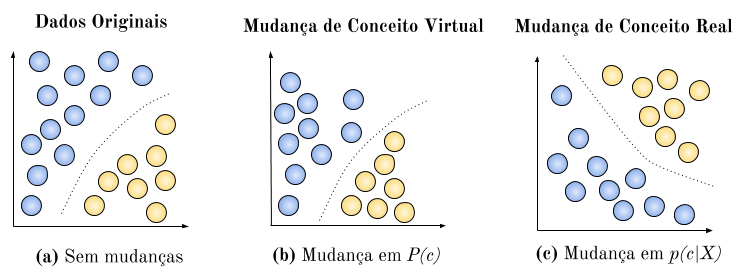
\includegraphics[scale=0.5]{../text/imagens/concept_drift.png}
        \caption{Mudança de Conceito Virtual vs. Mudança de Conceito Real}
        \label{fig:real_and_virtual_concept_drift}
    \end{center}
\end{figure}
\end{frame}

\begin{frame}{Mudança de Conceito}
    \begin{itemize}
        \item<1 -> As mudanças de conceito podem ocorrer de forma \alert{abrupta}, \alert{gradual}, \alert{incremental} ou \alert{recorrente} \cite{Zliobaite:2010}.
    \end{itemize}
    \begin{figure}[H]
        \begin{center}
            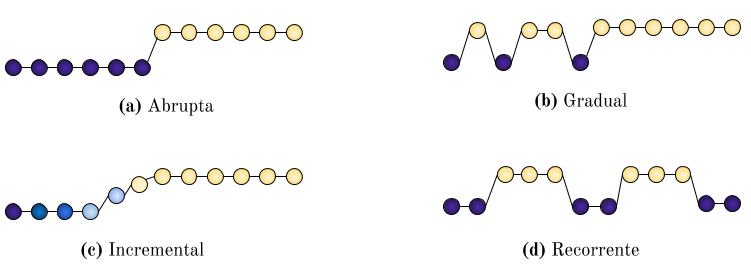
\includegraphics[scale=0.5]{imagens/concept_drift_patterns.png}
            \caption{Padrões de ocorrência de Mudanças de Conceito}
            \label{fig:concept_drift_patterns}
        \end{center}
    \end{figure}
\end{frame}

\begin{frame}{Mudança de Conceito}
    \begin{itemize}
        \item<1 -> O fenômeno mudança de conceito tem sido estudado em diferentes comunidades de pesquisa, sob diferentes nomeclaturas.
    \end{itemize}
    \begin{table}[!ht]
        \centering
        \resizebox{\textwidth}{!}{%
        \begin{tabular}[t]{ll}
        \toprule
        Área & Termos \\
        \midrule
        Mineração de Dados                  & Mudança de Conceito                        \\
        Aprendizado de Máquina              & Mudança de Conceito, Mudança de Covariável \\
        Computação Evolucionária            & Ambiente Evolutivo, Ambiente em Mudança    \\
        IA e Robótica                       & Ambiente Dinâmico                          \\
        Estatística, Séries Temporais      & Não Estacionário                           \\
        Recuperação de Informação           & Evolução Temporal                          \\
        \bottomrule
        \end{tabular}%
        }
        \caption{Terminologia - Mudança de Conceito \cite{Zliobaite:2010}}
        \label{tbl:taxonomy}
    \end{table}
\end{frame}

\begin{frame}{Mudança de Conceito}
    \begin{itemize}
        \item<1 -> Outra fonte comum de equívocos são os termos relacionados aos tipos de técnica de detecção.
    \end{itemize}

    \begin{table}[!ht]
        \centering
        \resizebox{\textwidth}{!}{%
        \begin{tabular}[t]{ll}
        \toprule
        Termo & Descrição \\
        \midrule
        Detecção de \textit{Outliers}      & Identificam padrões em desacordo com o esperado.                        \\
        Detecção de Novidades              & Identificam padrões ainda não observados. \\
        Detecção de \textit{Change Points} & Identificam variações abruptas de valor em séries temporais unidimensionais estacionárias.    \\
        Detecção de Mudança de Conceito    & Identificam alterações, na distribuição ou no contexto, que possam afetar a acurácia do modelo em uso. \\
        \bottomrule
        \end{tabular}%
        }
    \caption{Tipos de Técnicas de Detecção}
    \label{tbl:taxonomy_types_of_detection}
    \end{table}
\end{frame}

\begin{frame}{Algoritmos para Detecção de Mudança de Conceito}
    \begin{itemize}
        \item<1 -> Os algoritmos para Detecção de Mudanças de Conceito se dividem em duas categorias, conforme a necessidade de rotulação dos dados \cite{Zliobaite:2010}:
        \begin{itemize}
        \item<2 -> \alert{Explícitos/Supervisionados}: Dependem da rotulação dos dados, pois realizam a detecção a partir do monitoramento de medidas de performance como taxa de erro e acurácia.
        \item<3 -> \alert{Implícitos/Não Supervisionados}: Independem da rotulação dos dados, realizando a detecção através do monitoramento de características dos próprios dados ou de indicadores produzidos pelas técnicas de aprendizado aplicadas.
        \end{itemize}
    \end{itemize}
\end{frame}

\begin{frame}{Algoritmos para Detecção de Mudança de Conceito}
    \begin{itemize}
        \item<1 -> Os algoritmos \alert{Explícitos/Supervisionados} podem ser segmentados em três subcategorias \cite{Gama:2014:SCD:2597757.2523813}:
        \begin{itemize}
        \item<2 -> \alert{Métodos Baseados em Análise Sequencial}: Monitoram indicadores de performance. Mudança é identificada quando este valor atinge um limiar pré-estabelecido. Exemplos: \textit{Cumulative Sum (CUSUM)}, \textit{PageHinkley (PH)} \cite{Page:CUSUM:PageHinkley:1954} e \textit{Geometric Moving Average (GMA)} \cite{Roberts:2000:CCT:338441.338464}.
        \item<3 -> \alert{Abordagens baseadas em Estatística}: Identificam mudanças de conceito através da análise de parâmetros estatísticos associados aos resultados das predições. Exemplos: \textit{Drift Detection Method (DDM)} \cite{GamaMCR04}, \textit{Early Drift Detection Method (EDDM)} \cite{EDDM}, \textit{Exponentially Weighted Moving Average (EWMA)} \cite{Ross:2012:EWM:2076039.2076307} e \textit{Reactive Drift Detection Method (RDDM)} \cite{Barros:RDDM:2017}.
        \item<4 -> \alert{Métodos baseados em Janelas}: Comparam, continuamente, uma janela fixa com o sumário dos exemplos observados e uma janela deslizante com os dados mais recentes. Exemplos: \textit{Adaptive Windowing (ADWIN)} \cite{BifetG07}, \textit{SeqDrift} \cite{PearsSK14:SeqDrift:2014}, \textit{HDDMA} e \textit{HDDMW} \cite{BlancoCRBDM15:HDDMA:HDDMW:2015}.
        \end{itemize}
    \end{itemize}
\end{frame}

\begin{frame}{Algoritmos para Detecção de Mudança de Conceito}
    \begin{itemize}
        \item<1 -> Os algoritmos \alert{Implícitos/Não Supervisionados} também podem ser segmentados em três subcategorias \cite{GONCALVES20148144}:
        \begin{itemize}
        \item<2 -> \alert{Detecção de Novidade / Métodos de Agrupamento}: Utilizam técnicas derivadas dos métodos de agrupamento e de detecção de \textit{outliers}. Exemplos: \textit{OLINDDA} \cite{Spinosa:2007:OCA:1244002.1244107}, \textit{MINAS} \cite{Faria:2013:NDA:2480362.2480515}, \textit{Woo} \cite{Ryu:Kantardzic:2012}, \textit{DETECTNOD} \cite{Hashemi:Hayat:DETECTNOD:2010}, \textit{ECSMiner} \cite{Masud:2011:CNC:1978259.1978529} e \textit{GC3} \cite{Sethi2016b:GC3}.
        \item<3 -> \alert{Monitoramento de distribuição multivariada}: Monitoram diretamente a distribuição dos dados para cada atributo. Exemplos: \textit{CoC} \cite{Lee:Magoules:CoC:2012}, \textit{HDDDM} \cite{Ditzler:Polikar:HDDDM:2011}, \textit{PCA-detect} \cite{Kuncheva:PCADetect:20085}.
        \item<4 -> \alert{Monitoramento dependente de modelo}: Requerem a aplicação de um algoritmo de classificação probabilístico, pois as mudanças de conceito são detectadas a partir do monitoramento da probabilidade a posteriori. Exemplos: \textit{A-distance} \cite{Dredze:ADistance:2010585}, \textit{CDBD} \cite{Lindstrom:CDBD:2013} e \textit{Margin} \cite{Dries:Margin:2009}.
        \end{itemize}
    \end{itemize}
\end{frame}

\begin{frame}{Ferramenta: MOA}
    \begin{itemize}
        \item<1 -> Principal framework para mineração de dados em fluxos contínuos.
        \item<1 -> Permite implementar e validar novos métodos de detecção de mudança de conceito de forma trivial.
    \end{itemize}
    \begin{figure}[H]
        \begin{center}
            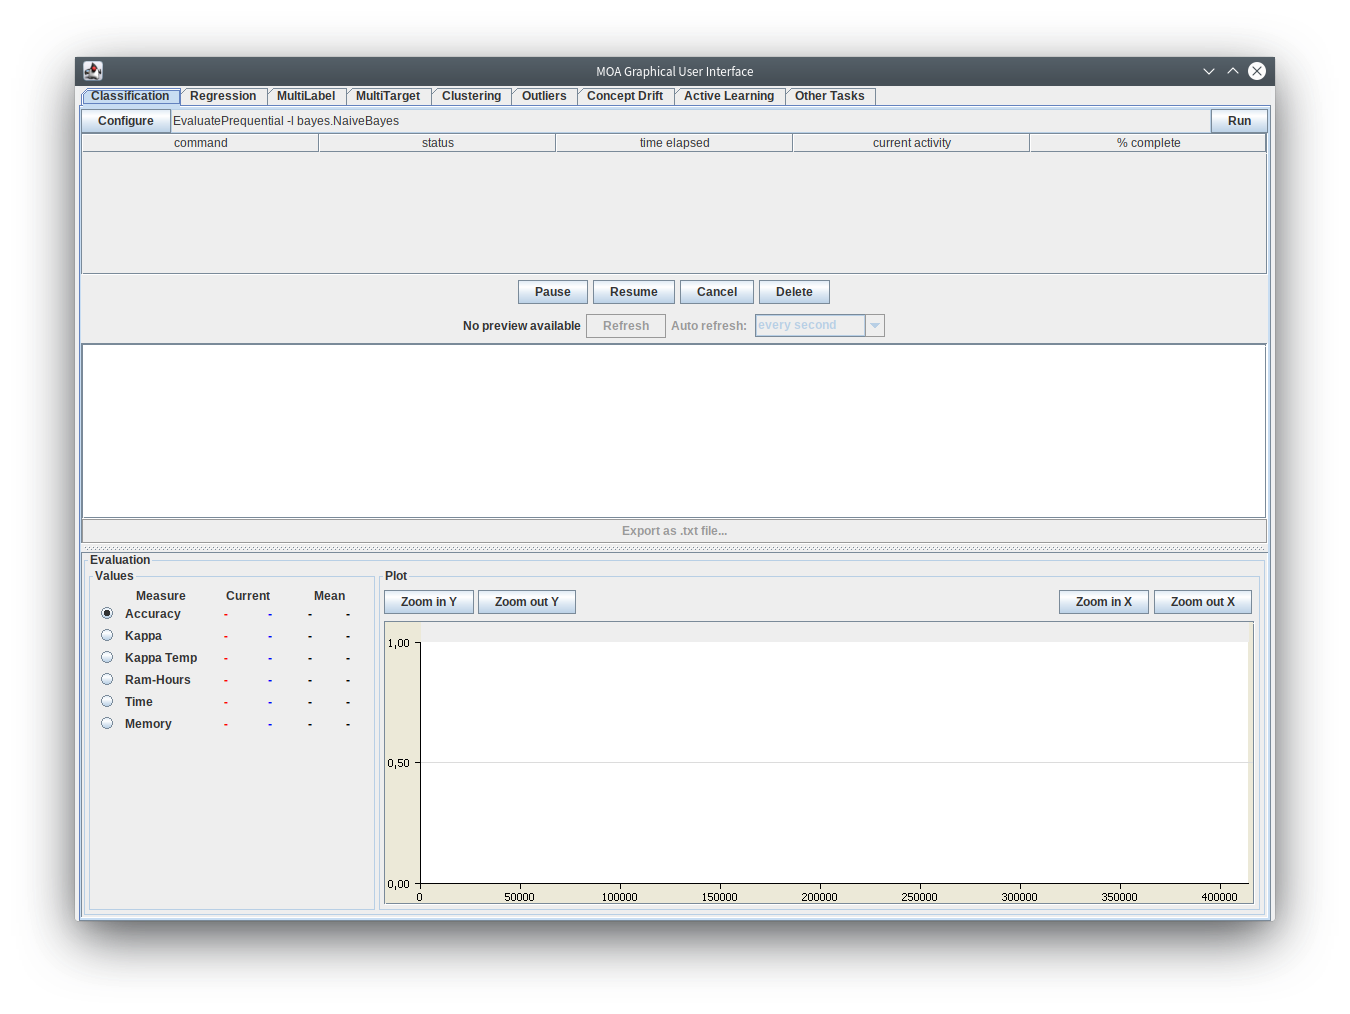
\includegraphics[scale=0.2]{imagens/moa.png}
            \caption{MOA - Tela Inicial}
            \label{fig:moa}
        \end{center}
    \end{figure}
\end{frame}

\begin{frame}{Ferramenta: Tornado}
    \begin{itemize}
        \item<1 -> Framework para avaliação de pares (classificador, detector de mudança de conceito).
    \end{itemize}
    \begin{figure}[ht]
        \begin{center}
            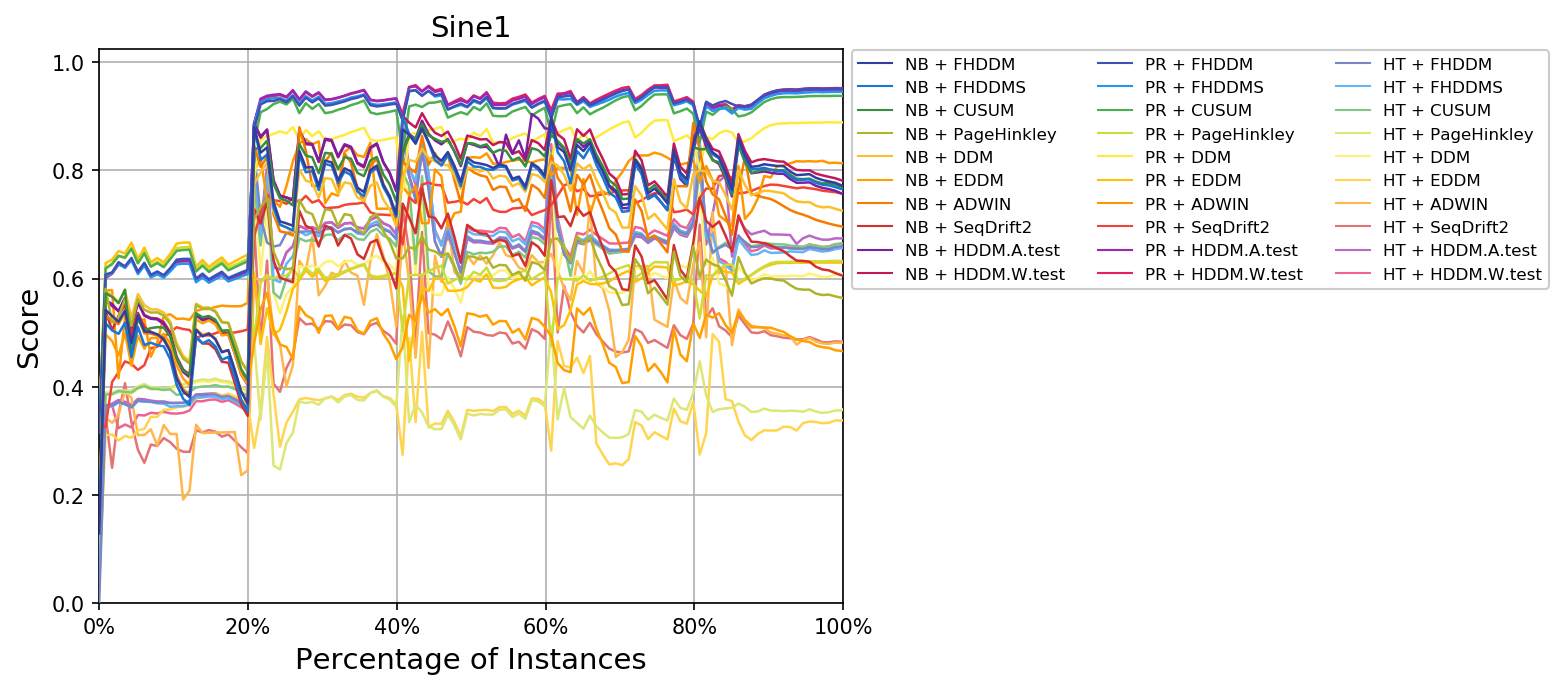
\includegraphics[width=\textwidth]{imagens/tornado_out2.png}
            \caption{Tornado - Exemplo de resultado \cite{Pesaranghader:Tornado}}
            \label{fig:tornado_out2}
        \end{center}
    \end{figure}
\end{frame}

%\subsection{Redes de Função de Base Radial}

\begin{frame}{Redes de Função de Base Radial}
    \begin{itemize}
        \item<1 -> \alert{Redes de Função de Base Radial} são redes neurais cujo principal diferencial é a forma de ativação, realizada através do cálculo da distância entre o dado e um centro definido \cite{Braga:RedesNeuraisTeoriaAplicacoes}.
        \item<2 -> A arquitetura de uma rede RBF, em sua forma mais básica, envolve três camadas: 
        \begin{itemize}
            \item<3 -> \alert{Entrada}: Recepciona os dados e encaminha para camada intermediária.
            \item<4 -> \alert{Intermediária}: Composta por funções de ativação de base radial que atuam como neurônios.
            \item<5 -> \alert{Saída}: Pondera os resultados da camada intermediária, agregando-os linearmente para compor a resposta final da rede.
        \end{itemize}
        \item<6 -> Na literatura, as funções Gaussianas são as funções de ativação mais usuais em redes RBF.
      \end{itemize}
\end{frame}

\begin{frame}{Redes de Função de Base Radial}
    \begin{figure}[H]
    \begin{center}
        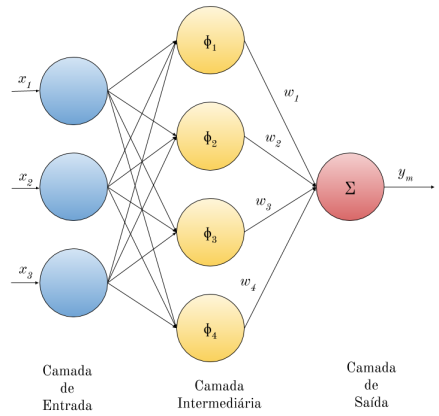
\includegraphics[scale=0.6]{../text/imagens/rbf_arq.png}
        \caption{Arquitetura RBF}
        \label{fig:rbg_arq}
    \end{center}
    \end{figure}
\end{frame}

%\subsection{Trabalhos Relacionados}

\begin{frame}{Trabalhos Relacionados}
    \begin{itemize}
        \item<1 -> Pesquisa na literatura em busca de trabalhos que propõem métodos para identificação de mudanças de conceito em fluxos contínuos de dados, de forma online e independente de rótulos. 
        \item<2 -> Também foram estudadas técnicas que pudessem subsidiar o desenvolvimento de novos algoritmos que atendam a esses requisitos.
    \end{itemize}
\end{frame}

\begin{frame}{Trabalhos Relacionados}
    \begin{itemize}
        \item<1 -> Análise dos algoritmos \alert{Implícitos/Não Supervisionados} da subcategoria \alert{Detecção de Novidade / Métodos de Agrupamento}.
        \item<2 -> Análise dos métodos para detecção de \textit{Change Points} em séries temporais que atuam de forma online:
        \begin{itemize}
            \item<2 -> Modelos autoregressivos;
            \item<2 -> Séries com autosimilaridade e periodicidade.
        \end{itemize}
        \item<3 -> Análise da aplicação de algoritmos de agrupamento estáveis.
        \item<4 -> Identificação de lacuna de pesquisa.
      \end{itemize}
\end{frame}

\section{Plano de Pesquisa}

%\subsection{Descrição do Problema}

\begin{frame}{Descrição do Problema}
    \begin{itemize}
        \item<1 -> O método proposto, denominado \textit{RBFDriftDetector}, utiliza as camadas inicial e intermediária da arquitetura básica de uma rede RBF, utilizando a Gaussiana como função de ativação.
        \item<2 -> Parâmetros: \textit{$\sigma$}, responsável por limitar o raio da radial, e \textit{$\lambda$}, que define um limiar para ativação de um centro.
      \end{itemize}
\end{frame}
 

\begin{frame}{Descrição do Problema}
    \begin{figure}[H]
        \begin{center}
            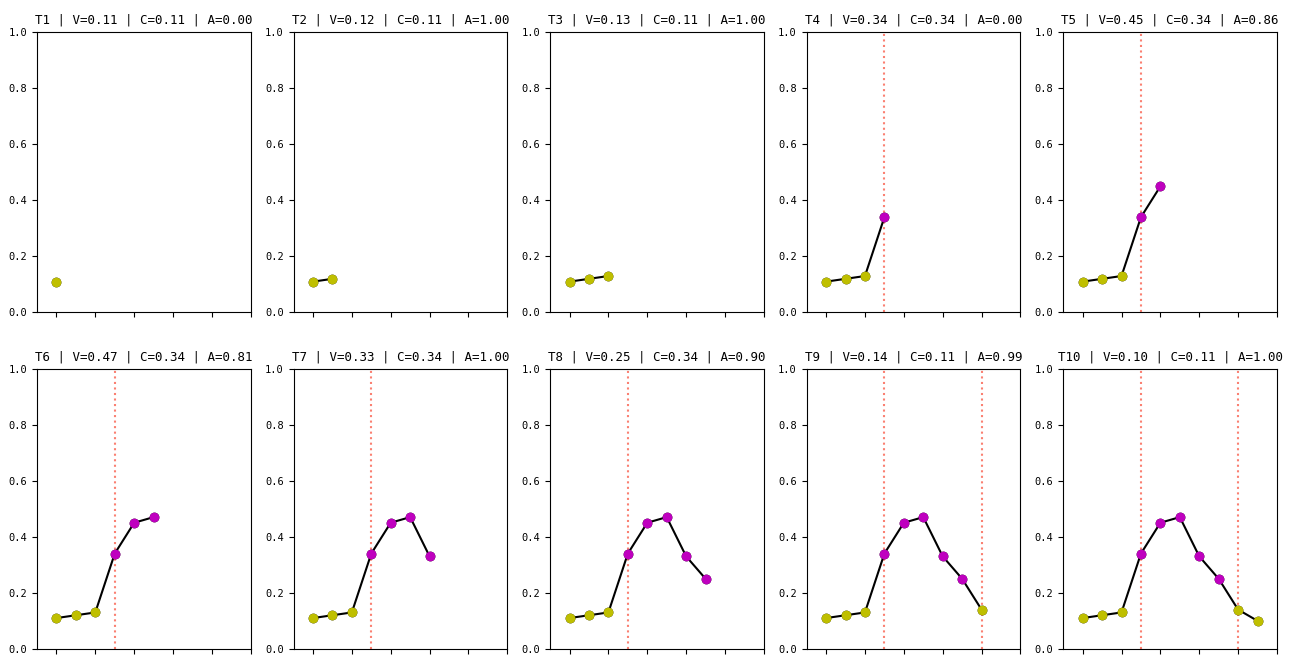
\includegraphics[width=\textwidth]{../text/imagens/funcionamento_algoritmo.png}
            \caption{Exemplo de funcionamento do algoritmo}
            \label{fig:funcionamento_algoritmo}
        \end{center}
    \end{figure}
\end{frame}

%\subsection{Atividades de Pesquisa}

\begin{frame}{Atividades de Pesquisa}
    \begin{table}[ht]
        \begin{center}
        \resizebox{\textwidth}{!}{ % abre resizebox, setar tabela da largura da página.
        \begin{tabular}{|c|l|l|l|l|l|l|l|l|l|l|l|l|l|l|l|l|l|l|l|l|l|l|l|l|}
        \hline
        \multicolumn{1}{|c|}{\multirow{2}{*}{Atividades}} & \multicolumn{24}{c|}{Meses} \\ \cline{2-25}
        \multicolumn{1}{|c|}{} & 01 & 02 & 03 & 04 & 05 & 06 & 07 & 08 & 09 & 10 & 11 & 12 & 13 & 14 & 15 & 16 & 17 & 18 & 19 & 20 & 21 & 22 & 23 & 24 \\ \hline
        %\rowcolor[HTML]{EFEFEF}
        
        1-Disciplinas & X & X & X & X & X & X & X & X & X & X & ~ & ~ & ~ & ~ & ~ & ~ & ~ & ~ & ~ & ~ & ~ & ~ & ~ & ~ \\ \hline
        2-Revisão da Literatura & ~ & ~ & ~ & ~ & ~ & ~ & X & X & X & X & X & X & ~ & ~ & ~ & ~ &  ~ & ~ & ~ & ~ & ~ & ~ & ~ & ~ \\ \hline
        3-Experimentos  & ~ & ~ & ~ & ~ & ~ & ~ & ~ & ~ & X & X & X  & X & $\bullet$ & $\bullet$ & $\bullet$ & $\bullet$ & ~ & ~ & ~ & ~ & ~ & ~ & ~ & ~ \\ \hline
        4-Análise dos Resultados & ~ & ~ & ~ & ~ & ~ & ~ & ~ & ~ & ~ & ~ & X & X & ~  & ~  & ~ & $\bullet$ & $\bullet$ & $\bullet$ & ~ & ~ & ~ & ~ & ~ & ~ \\ \hline
        5-Escrita da qualificação & ~ & ~ & ~ & ~ & ~ & ~ & ~ & ~ & ~ & X & X & X & ~ & ~ & ~ & ~ & ~ & ~ & ~ & ~ & ~ & ~ & ~ & ~ \\ \hline
        6-Estágio docente & ~ & ~ & ~ & ~ & ~ & ~ & ~ & ~ & ~ & ~ & ~ & ~ & ~ & ~ & ~ & $\bullet$ & $\bullet$ & $\bullet$ & $\bullet$ & $\bullet$ & $\bullet$ & ~ & ~ & ~ \\ \hline
        7-Pesquisa Orientada & ~ & ~ & ~ & ~ & ~ & ~ & X & X & X & X & X & X & $\bullet$ & $\bullet$ & $\bullet$ & $\bullet$ & $\bullet$ & $\bullet$ & $\bullet$ & $\bullet$ & $\bullet$ & $\bullet$ & $\bullet$ & $\bullet$ \\ \hline
        8-Apresentação da qualificação & ~ & ~ & ~ & ~ & ~ & ~ & ~ & ~ & ~ & ~ & ~ & ~ & $\bullet$ & ~ & ~ & ~ & ~ & ~ & ~ & ~ & ~ & ~ & ~ & ~ \\ \hline
        9-Escrita de artigos& ~ & ~ & ~ & ~ & ~ & ~ & ~ & ~ & ~ & ~ & ~ & ~ & ~  & ~ & ~ & ~ & ~ & $\bullet$ & $\bullet$ & ~ & ~ & ~ & ~ & ~ \\ \hline
        10-Escrita da dissertação& ~ & ~ & ~ & ~ & ~ & ~ & ~ & ~ & ~ & X & X & X & ~ & ~ & ~ & ~ & $\bullet$ & $\bullet$ & $\bullet$ & $\bullet$ & $\bullet$ & $\bullet$ & $\bullet$ & $\bullet$ \\ \hline
        11- Defesa da dissertação& ~ & ~ & ~ & ~ & ~ & ~ & ~ & ~ & ~ & ~ & ~ & ~ & ~ & ~ & ~ & ~ & ~ & ~ & ~ & ~ & ~ & ~ & ~ & $\bullet$ \\ \hline
        
        \hline
        \end{tabular}
        } % fecha resizebox
        \caption{Cronograma de atividades}     % mude aqui para seu título da tabela
        \label{cronograma} % para referencia no texto.
        \end{center}
    \end{table}
\end{frame}

\section{Experimentos Iniciais}

\begin{frame}{Configuração dos Experimentos}
    \begin{itemize}
        \item<1 -> Conjuntos de dados sintéticos construídos através de especializações das classes geradoras do MOA.
        \item<2 -> As classes geradoras originais foram alteradas para permitir a inclusão de ruídos com distribuição uniforme e corrigir limitações.
        \item<3 -> Cada conjunto de dados é composto por \alert{$2.500$} observações, com valores \alert{entre $0$ e $1$} e conceitos compostos por \alert{$400$} registros.
      \end{itemize}
\end{frame}

\begin{frame}{Configuração dos Experimentos}
      \begin{center} 
        \begin{table}[h]
        \resizebox{\textwidth}{!} {%
        \begin{tabular}{llllm{7.5cm}}
        \toprule
        Conjunto & Classe utilizada & Qtd. Observações & Tamanho Conceito & Ruído \\
        \midrule
        Mudanças Abruptas          & \textit{AbruptChangeGenerator}  & $2.500$ & $400$ & $[-0.1, 0.2]$  \\
        Mudanças Graduais          & \textit{GradualChangeGenerator} & $2.500$ & $400$ & -  \\
        Sem Mudanças               & \textit{NoChangeGenerator}      & $2.500$ & -     & $[-0.1, 0.2]$  \\
        \bottomrule
        \end{tabular}
        }
        \caption{Conjuntos de dados produzidos}
        \label{tbl:configuracao_tarefa}
        \end{table}
    \end{center}
\end{frame}

\begin{frame}{Configuração dos Experimentos}
    \begin{itemize}
        \item<1 -> Parametrização da classe de avaliação utilizada.
      \end{itemize}
      \begin{center} 
        \begin{table}[h]
        \resizebox{\textwidth}{!} {%
        \begin{tabular}{llm{7.5cm}}
        \toprule
        Parâmetro & Valor & Observação \\
        \midrule
        learner          & ChangeDetectorLearner  &  O algoritmo de detecção de mudanças de conceito a ser testado é definido no atributo \textit{driftDetectionMethod} da classe \textit{ChangeDetectorLearner}.                   \\
        stream           & ARFFFileStream         &  Caminho para um dos arquivos \textit{ARFF} descrito na seção anterior. O atributo \textit{classIndex} deve ser definido como $0$, pois não existem rótulos nestes conjuntos de dados.  \\ 
        instanceLimit    & $-1$                            &  Desabilita o limite de instâncias a serem processadas.  \\
        timeLimit        & $-1$                            &  Desabilita o limite de tempo de execução.  \\ 
        sampleFrequency  & \hspace{3mm}$1$                 &  Uma linha de resultado do avaliador deve ser gerada para cada instância processada.  \\
        \bottomrule
        \end{tabular}
        }
        \caption{Configuração da classe \textit{BasicConceptDriftPerformanceEvaluator}}
        \label{tbl:configuracao_tarefa}
        \end{table}
    \end{center}
\end{frame}

\begin{frame}{Configuração dos Experimentos}
    \begin{itemize}
        \item<1 -> Indicadores de avaliação analisados.
      \end{itemize}
      \begin{center} 
        \begin{table}[h]
        \resizebox{\textwidth}{!} {%
        \begin{tabular}{lm{10cm}}
        \toprule
        Indicador & Observação \\
        \midrule
        Tempo de Processamento    &  Tempo médio (seg.) de processamento por instância. \\
        Mudanças Existentes       &  Quantidade de mudanças existentes. \\
        Mudanças Detectadas       &  Quantidade de mudanças detectadas corretamente. \\
        Falso-positivos           &  Quantidade de mudanças detecatadas erroneamente. \\  
        Atraso de Detecção        &  Quantidade média de instâncias até a detecção. \\
        \bottomrule
        \end{tabular}
        }
        \caption{Indicadores analisados}
        \label{tbl:indicadores_analisado}
        \end{table}
    \end{center}
\end{frame}

\begin{frame}{Configuração dos Experimentos}
    \begin{itemize}
        \item<1 -> Algoritmos comparados e os parâmetros utilizados.
      \end{itemize}
      \begin{center} 
        \begin{table}[ht]
        \resizebox{\textwidth}{!} {%
        \begin{tabular}{lm{10cm}}
        \toprule
        Algoritmo & Parâmetros \\
        \midrule
        RBFDriftDetector          &  $\sigma = 2$; $\lambda = 0.5$ \\
        CUSUM                     &  $MinNumInstances = 30; \delta = 0.005; \lambda = 50$ \\
        PageHinkley               &  $MinNumInstances = 30; \delta = 0.005; \lambda = 50; \alpha = 1$ \\
        ADWIN                     &  $\delta = 0.002$ \\
        \bottomrule
        \end{tabular}
        }
        \caption{Parâmetros utilizados para cada algoritmo}
        \label{tbl:parametros_algoritmos}
        \end{table}
    \end{center}
\end{frame}

\begin{frame}{Pettitt}
    \begin{itemize}
        \item<1 -> Implementação do teste não paramétrico de Pettitt como método para detecção de mudanças de conceito \cite{Pettitt}.
    \end{itemize}
      \begin{center} 
        \begin{table}[H]
        \resizebox{\textwidth}{!} {%
        \begin{tabular}{llllll}
        \toprule
        Conjunto de Dados & Tempo de processamento & Mudanças Existentes & Mudanças Detectadas & Falso-positivos & Atraso de Detecção \\
        \midrule
        Sem mudanças           &  $3.19$ & $0$ & $0$ & $4$ & $-$ \\
        Mudanças Abruptas      &  $2.09$ & $6$ & $3$ & $2$ & $132$ \\
        Mudanças Incrementais  &  $1.48$ & $6$ & $4$ & $2$ & $133$ \\
        \bottomrule
        \end{tabular}
        }
        \caption{Resultados - Método de Pettitt}
        \label{tbl:pettitt}
        \end{table}
    \begin{itemize}
        \item<2 -> Propenso à produção de falso-positivos e computacionalmente ineficiente.
    \end{itemize}
    \end{center}
\end{frame}

% Exp 1
\begin{frame}{Experimento 1 - Fluxo sem mudanças de conceito}
    \begin{itemize}
        \item<1 -> Experimento realizado utilizando o conjunto de dados \alert{\textbf{sem} mudanças de conceito}, visando avaliar a tendência de produção de falso-positivos.
    \end{itemize}
    \begin{center} 
        \begin{table}[H]
        \resizebox{\textwidth}{!} {%
        \begin{tabular}{llllll}
        \toprule
        Algoritmo & Tempo de processamento & Mudanças Existentes & Mudanças Detectadas & Falso-positivos & Atraso de Detecção \\
        \midrule
        RBFDriftDetector          &  $0.22$ & $0$ & $0$ & $0$ & $-$ \\
        CUSUM                     &  $0.31$ & $0$ & $0$ & $0$ & $-$ \\
        PageHinkley               &  $0.24$ & $0$ & $0$ & $0$ & $-$ \\
        ADWIN                     &  $0.21$ & $0$ & $0$ & $0$ & $-$ \\
        \bottomrule
        \end{tabular}
        }
        \caption{Experimento 1 - Fluxo sem mudanças de conceito}
        \label{tbl:exp1}
        \end{table}
    \end{center}
    \begin{itemize}
        \item<2 -> Todos algoritmos testados demonstraram tolerância a ruídos e baixa propensão a identificar falso-positivos.
        \item<3 -> O algoritmo proposto obteve a segunda melhor performance, superado pelo ADWIN por uma pequena margem.
    \end{itemize}
\end{frame}

\begin{frame}{Experimento 1 - Fluxo sem mudanças de conceito}
\begin{figure}[ht]
    \begin{center}
        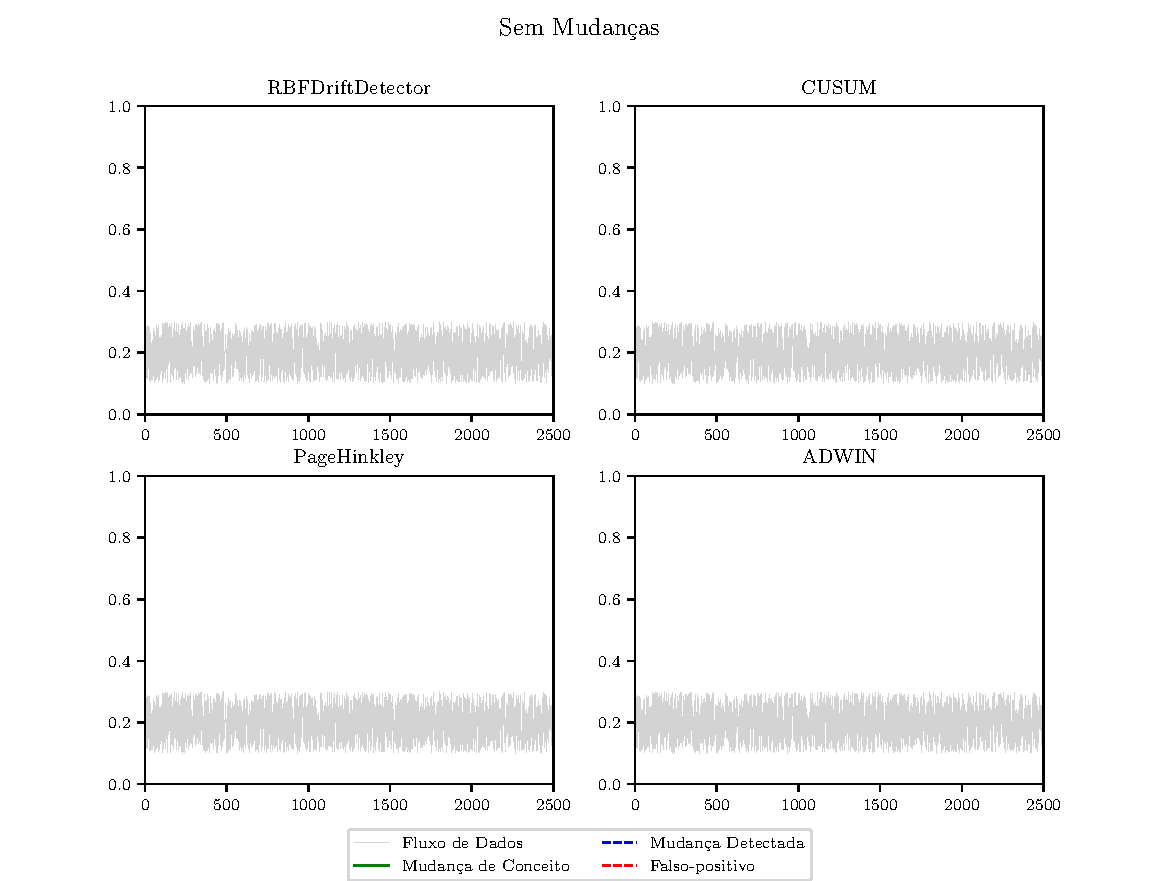
\includegraphics[scale=0.45]{../text/imagens/nochange.pdf}
        \caption{Representação Gráfica - Sem mudanças de conceito}
        \label{fig:exp_sem_mudancas}
    \end{center}
\end{figure}
\end{frame}

% Exp 2
\begin{frame}{Experimento 2 - Fluxo com mudanças de conceito abruptas}
    \begin{itemize}
        \item<1 -> Experimento realizado utilizando o conjunto de dados \alert{com mudanças de conceito \textbf{abruptas}}.
    \end{itemize}
    \begin{center} 
        \begin{table}[H]
        \resizebox{\textwidth}{!} {%
        \begin{tabular}{llllll}
        \toprule
        Algoritmo & Tempo de processamento & Mudanças Existentes & Mudanças Detectadas & Falso-positivos & Atraso de Detecção \\
        \midrule
        RBFDriftDetector          &  $0.23$ & $6$ & $6$    & $0$    & $1$ \\
        CUSUM                     &  $0.29$ & $6$ & $3$    & $0$    & $68$ \\
        PageHinkley               &  $0.22$ & $6$ & $1$    & $0$    & $17$ \\
        ADWIN                     &  $0.21$ & $6$ & $6$    & $2046$ & $9$ \\
        \bottomrule
        \end{tabular}
        }
        \caption{Experimento 2 - Fluxo com mudanças de conceito abruptas}
        \label{tbl:exp2}
        \end{table}
    \end{center}
    \begin{itemize}
        \item<2 -> Método proposto identificou todas mudanças, sem falso-positivos e com menor atraso de detecção.
    \end{itemize}
\end{frame}

\begin{frame}{Experimento 2 - Fluxo com mudanças de conceito abruptas}
    \begin{figure}[H]
        \begin{center}
            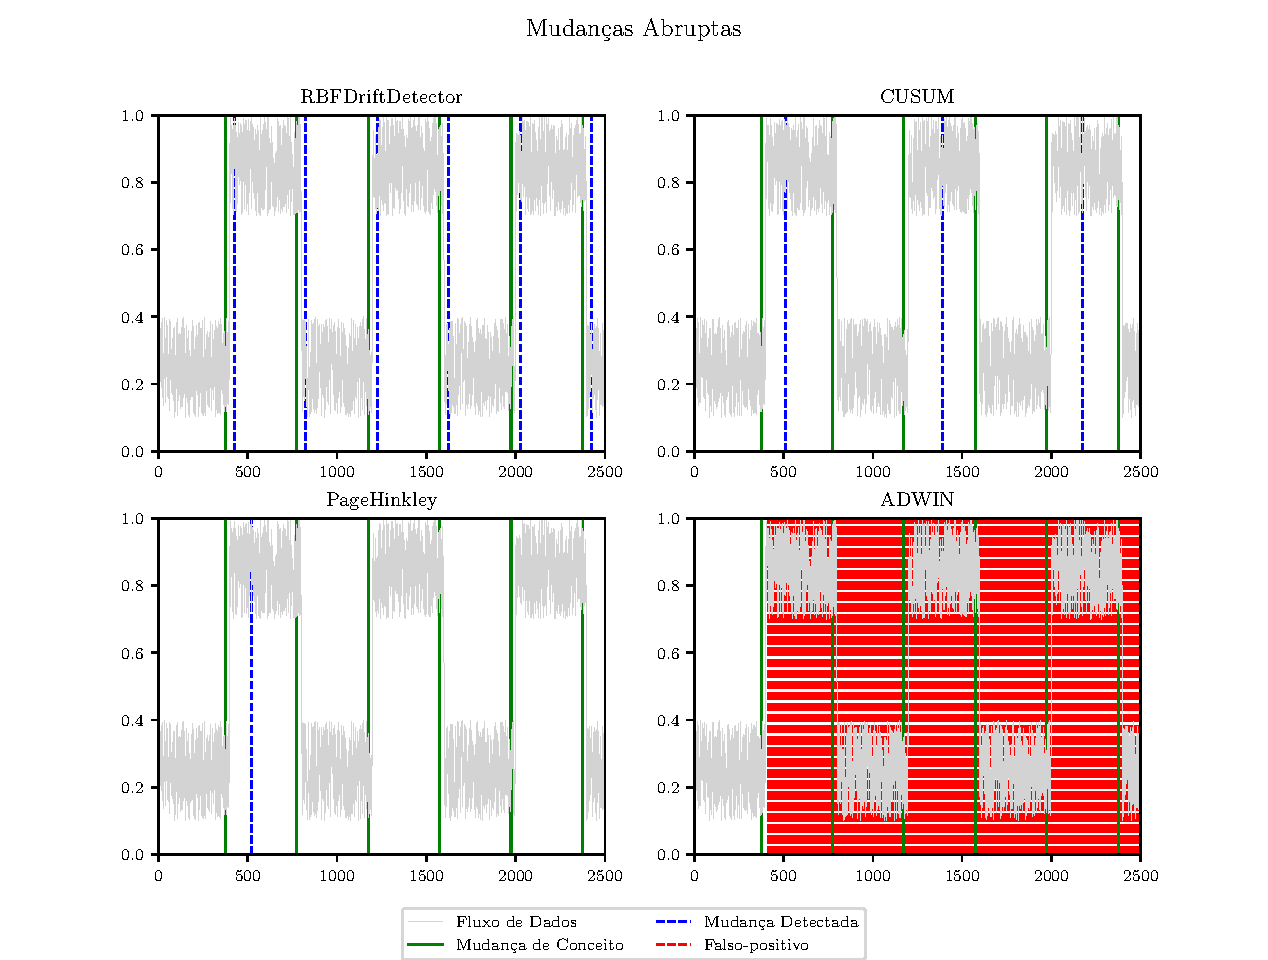
\includegraphics[scale=0.45]{../text/imagens/abrupt.pdf}
            \caption{Representação Gráfica - Mudanças Abruptas}
            \label{fig:exp_abrupta}
        \end{center}
    \end{figure}
\end{frame}

% Exp 3
\begin{frame}{Experimento 3 - Fluxo com mudanças de conceito graduais}
    \begin{itemize}
        \item<1 -> Experimento realizado utilizando o conjunto de dados \alert{com mudanças de conceito \textbf{graduais}}.
    \end{itemize}
    \begin{center} 
        \begin{table}[ht]
        \resizebox{\textwidth}{!} {%
        \begin{tabular}{llllll}
        \toprule
        Algoritmo & Tempo de processamento & Mudanças Existentes & Mudanças Detectadas & Falso-positivos & Atraso de Detecção \\
        \midrule
        RBFDriftDetector          &  $0.24$ & $6$ & $5$    & $1$    & $171$ \\
        CUSUM                     &  $0.65$ & $6$ & $3$    & $0$    & $32$ \\
        PageHinkley               &  $0.26$ & $6$ & $1$    & $0$    & $4$ \\
        ADWIN                     &  $0.27$ & $6$ & $6$ & $2238$ & $1$ \\
        \bottomrule
        \end{tabular}
        }
        \caption{Experimento 3 - Fluxo com mudanças de conceito graduais}
        \label{tbl:exp3}
        \end{table}
    \end{center}
    \begin{itemize}
        \item<2 -> Método proposto identificou 5 das 6 mudanças existentes e sinalizou um falso-positivo.
        \item<3 -> Obteve a melhor acurácia, apesar de apresentar a maior taxa de atraso.
    \end{itemize}
\end{frame}

\begin{frame}{Experimento 3 - Fluxo com mudanças de conceito graduais}
    \begin{figure}[ht]
        \begin{center}
            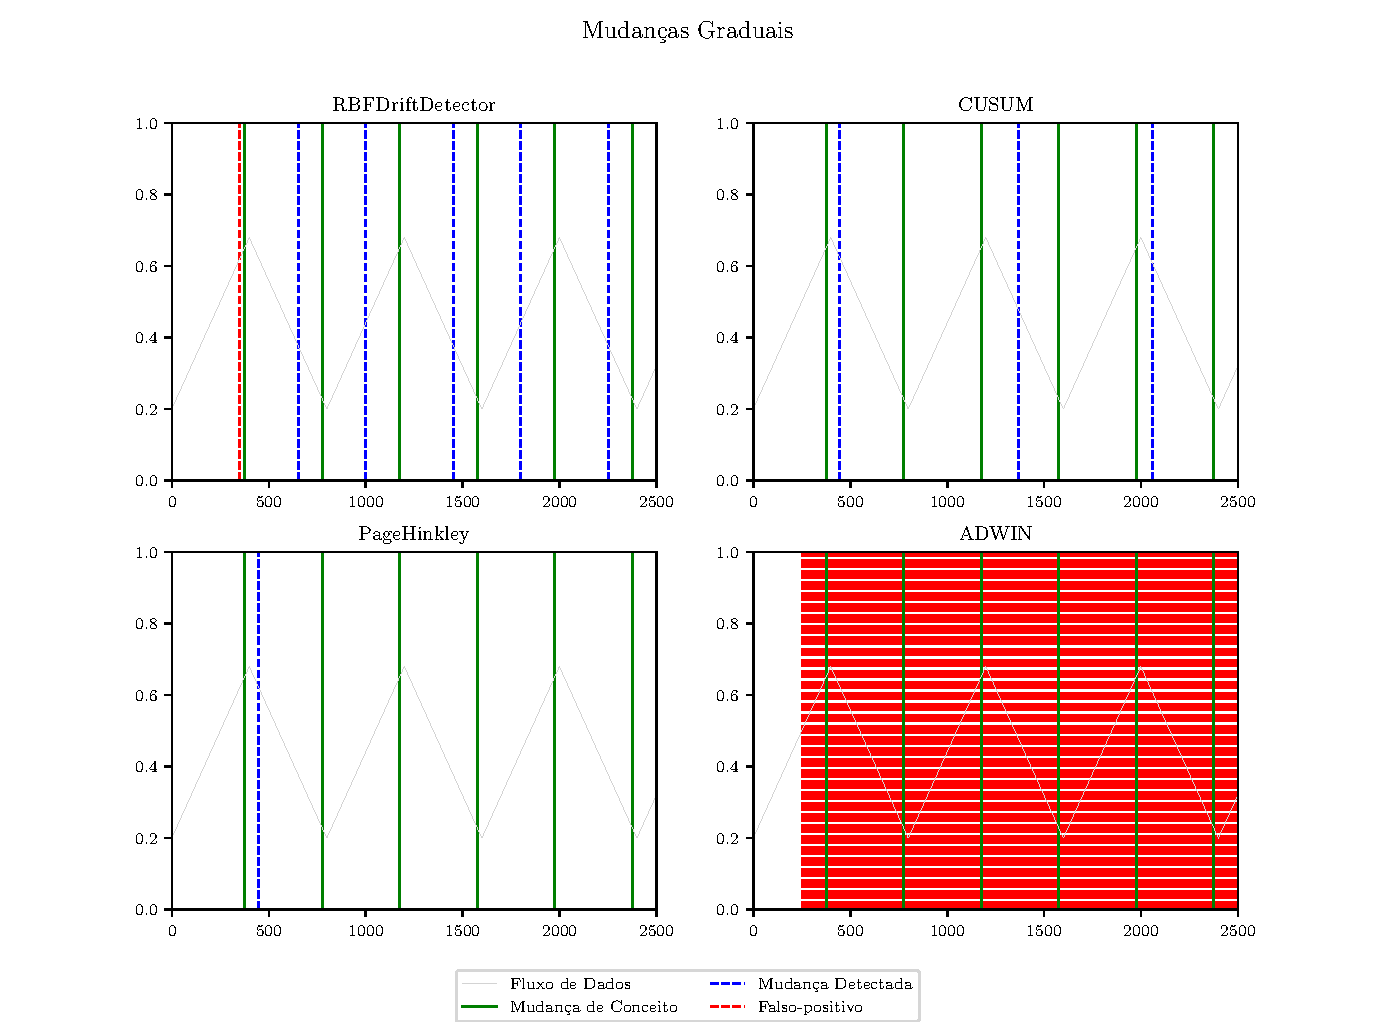
\includegraphics[scale=0.45]{../text/imagens/gradual.pdf}
            \caption{Representação Gráfica - Mudanças Graduais}
            \label{fig:exp_gradual}
        \end{center}
        \end{figure}
\end{frame}

\section{Conclusão}

\begin{frame}{Conclusão}
    \begin{itemize}
        \item<1 -> Algoritmo apresenta bom desempenho e acurácia.
        \item<2 -> Método proposto pode ser aprimorado para detecção de mudanças graduais.
        \item<3 -> Os resultados obtidos, apesar de preliminares, mostraram-se promissores, indicando que o tema de pesquisa deve continuar a ser investigado.
      \end{itemize}
\end{frame}

\begin{frame}{Trabalhos Futuros}
    \begin{itemize}
        \item<1 -> Realizar experimentos com fluxos recorrentes e incrementais.
        \item<1 -> Integrar uma cadeia de Markov ao método proposto, permitindo a análise do comportamento das mudanças e o aprimoramento da acurácia das detecções.
        \item<1 -> Implementar os algoritmos OLINDDA, MINAS e DETECNOD para serem comparados.
        \item<1 -> Implementar e validar o algoritmo no framework Tornado.
        \item<1 -> Alterar o algoritmo para permitir que o centro se desloque dentro do grupo formado.
      \end{itemize}
\end{frame}

% \begin{frame}[fragile]{Metropolis}

%   The \themename theme is a Beamer theme with minimal visual noise
%   inspired by the \href{https://github.com/hsrmbeamertheme/hsrmbeamertheme}{\textsc{hsrm} Beamer
%   Theme} by Benjamin Weiss.

%   Enable the theme by loading

%   \begin{verbatim}    \documentclass{beamer}
%     \usetheme{metropolis}\end{verbatim}

%   Note, that you have to have Mozilla's \emph{Fira Sans} font and XeTeX
%   installed to enjoy this wonderful typography.
% \end{frame}
% \begin{frame}[fragile]{Sections}
%   Sections group slides of the same topic

%   \begin{verbatim}    \section{Elements}\end{verbatim}

%   for which \themename provides a nice progress indicator \ldots
% \end{frame}

% \section{Titleformats}

% \begin{frame}{Metropolis titleformats}
% 	\themename supports 4 different titleformats:
% 	\begin{itemize}
% 		\item Regular
% 		\item \textsc{Smallcaps}
% 		\item \textsc{allsmallcaps}
% 		\item ALLCAPS
% 	\end{itemize}
% 	They can either be set at once for every title type or individually.
% \end{frame}

% {
%     \metroset{titleformat frame=smallcaps}
% \begin{frame}{Small caps}
% 	This frame uses the \texttt{smallcaps} titleformat.

% 	\begin{alertblock}{Potential Problems}
% 		Be aware, that not every font supports small caps. If for example you typeset your presentation with pdfTeX and the Computer Modern Sans Serif font, every text in smallcaps will be typeset with the Computer Modern Serif font instead.
% 	\end{alertblock}
% \end{frame}
% }

% {
% \metroset{titleformat frame=allsmallcaps}
% \begin{frame}{All small caps}
% 	This frame uses the \texttt{allsmallcaps} titleformat.

% 	\begin{alertblock}{Potential problems}
% 		As this titleformat also uses smallcaps you face the same problems as with the \texttt{smallcaps} titleformat. Additionally this format can cause some other problems. Please refer to the documentation if you consider using it.

% 		As a rule of thumb: Just use it for plaintext-only titles.
% 	\end{alertblock}
% \end{frame}
% }

% {
% \metroset{titleformat frame=allcaps}
% \begin{frame}{All caps}
% 	This frame uses the \texttt{allcaps} titleformat.

% 	\begin{alertblock}{Potential Problems}
% 		This titleformat is not as problematic as the \texttt{allsmallcaps} format, but basically suffers from the same deficiencies. So please have a look at the documentation if you want to use it.
% 	\end{alertblock}
% \end{frame}
% }

% \section{Elements}

% \begin{frame}[fragile]{Typography}
%       \begin{verbatim}The theme provides sensible defaults to
% \emph{emphasize} text, \alert{accent} parts
% or show \textbf{bold} results.\end{verbatim}

%   \begin{center}becomes\end{center}

%   The theme provides sensible defaults to \emph{emphasize} text,
%   \alert{accent} parts or show \textbf{bold} results.
% \end{frame}

% \begin{frame}{Font feature test}
%   \begin{itemize}
%     \item Regular
%     \item \textit{Italic}
%     \item \textsc{SmallCaps}
%     \item \textbf{Bold}
%     \item \textbf{\textit{Bold Italic}}
%     \item \textbf{\textsc{Bold SmallCaps}}
%     \item \texttt{Monospace}
%     \item \texttt{\textit{Monospace Italic}}
%     \item \texttt{\textbf{Monospace Bold}}
%     \item \texttt{\textbf{\textit{Monospace Bold Italic}}}
%   \end{itemize}
% \end{frame}

% \begin{frame}{Lists}
%   \begin{columns}[T,onlytextwidth]
%     \column{0.33\textwidth}
%       Items
%       \begin{itemize}
%         \item Milk \item Eggs \item Potatos
%       \end{itemize}

%     \column{0.33\textwidth}
%       Enumerations
%       \begin{enumerate}
%         \item First, \item Second and \item Last.
%       \end{enumerate}

%     \column{0.33\textwidth}
%       Descriptions
%       \begin{description}
%         \item[PowerPoint] Meeh. \item[Beamer] Yeeeha.
%       \end{description}
%   \end{columns}
% \end{frame}
% \begin{frame}{Animation}
%   \begin{itemize}[<+- | alert@+>]
%     \item \alert<4>{This is\only<4>{ really} important}
%     \item Now this
%     \item And now this
%   \end{itemize}
% \end{frame}
% \begin{frame}{Figures}
%   \begin{figure}
%     \newcounter{density}
%     \setcounter{density}{20}
%     \begin{tikzpicture}
%       \def\couleur{alerted text.fg}
%       \path[coordinate] (0,0)  coordinate(A)
%                   ++( 90:5cm) coordinate(B)
%                   ++(0:5cm) coordinate(C)
%                   ++(-90:5cm) coordinate(D);
%       \draw[fill=\couleur!\thedensity] (A) -- (B) -- (C) --(D) -- cycle;
%       \foreach \x in {1,...,40}{%
%           \pgfmathsetcounter{density}{\thedensity+20}
%           \setcounter{density}{\thedensity}
%           \path[coordinate] coordinate(X) at (A){};
%           \path[coordinate] (A) -- (B) coordinate[pos=.10](A)
%                               -- (C) coordinate[pos=.10](B)
%                               -- (D) coordinate[pos=.10](C)
%                               -- (X) coordinate[pos=.10](D);
%           \draw[fill=\couleur!\thedensity] (A)--(B)--(C)-- (D) -- cycle;
%       }
%     \end{tikzpicture}
%     \caption{Rotated square from
%     \href{http://www.texample.net/tikz/examples/rotated-polygons/}{texample.net}.}
%   \end{figure}
% \end{frame}
% \begin{frame}{Tables}
%   \begin{table}
%     \caption{Largest cities in the world (source: Wikipedia)}
%     \begin{tabular}{lr}
%       \toprule
%       City & Population\\
%       \midrule
%       Mexico City & 20,116,842\\
%       Shanghai & 19,210,000\\
%       Peking & 15,796,450\\
%       Istanbul & 14,160,467\\
%       \bottomrule
%     \end{tabular}
%   \end{table}
% \end{frame}
% \begin{frame}{Blocks}
%   Three different block environments are pre-defined and may be styled with an
%   optional background color.

%   \begin{columns}[T,onlytextwidth]
%     \column{0.5\textwidth}
%       \begin{block}{Default}
%         Block content.
%       \end{block}

%       \begin{alertblock}{Alert}
%         Block content.
%       \end{alertblock}

%       \begin{exampleblock}{Example}
%         Block content.
%       \end{exampleblock}

%     \column{0.5\textwidth}

%       \metroset{block=fill}

%       \begin{block}{Default}
%         Block content.
%       \end{block}

%       \begin{alertblock}{Alert}
%         Block content.
%       \end{alertblock}

%       \begin{exampleblock}{Example}
%         Block content.
%       \end{exampleblock}

%   \end{columns}
% \end{frame}
% \begin{frame}{Math}
%   \begin{equation*}
%     e = \lim_{n\to \infty} \left(1 + \frac{1}{n}\right)^n
%   \end{equation*}
% \end{frame}
% \begin{frame}{Line plots}
%   \begin{figure}
%     \begin{tikzpicture}
%       \begin{axis}[
%         mlineplot,
%         width=0.9\textwidth,
%         height=6cm,
%       ]

%         \addplot {sin(deg(x))};
%         \addplot+[samples=100] {sin(deg(2*x))};

%       \end{axis}
%     \end{tikzpicture}
%   \end{figure}
% \end{frame}
% \begin{frame}{Bar charts}
%   \begin{figure}
%     \begin{tikzpicture}
%       \begin{axis}[
%         mbarplot,
%         xlabel={Foo},
%         ylabel={Bar},
%         width=0.9\textwidth,
%         height=6cm,
%       ]

%       \addplot plot coordinates {(1, 20) (2, 25) (3, 22.4) (4, 12.4)};
%       \addplot plot coordinates {(1, 18) (2, 24) (3, 23.5) (4, 13.2)};
%       \addplot plot coordinates {(1, 10) (2, 19) (3, 25) (4, 15.2)};

%       \legend{lorem, ipsum, dolor}

%       \end{axis}
%     \end{tikzpicture}
%   \end{figure}
% \end{frame}
% \begin{frame}{Quotes}
%   \begin{quote}
%     Veni, Vidi, Vici
%   \end{quote}
% \end{frame}

% {%
% \setbeamertemplate{frame footer}{My custom footer}
% \begin{frame}[fragile]{Frame footer}
%     \themename defines a custom beamer template to add a text to the footer. It can be set via
%     \begin{verbatim}\setbeamertemplate{frame footer}{My custom footer}\end{verbatim}
% \end{frame}
% }

% \begin{frame}{References}
%   Some references to showcase [allowframebreaks] \cite{knuth92,ConcreteMath,Simpson,Er01,greenwade93}
% \end{frame}

% \section{Conclusion}

% \begin{frame}{Summary}

%   Get the source of this theme and the demo presentation from

%   \begin{center}\url{github.com/matze/mtheme}\end{center}

%   The theme \emph{itself} is licensed under a
%   \href{http://creativecommons.org/licenses/by-sa/4.0/}{Creative Commons
%   Attribution-ShareAlike 4.0 International License}.

%   \begin{center}\ccbysa\end{center}

% \end{frame}

% \begin{frame}[standout]
%   Questions?
% \end{frame}

% \appendix

% \begin{frame}[fragile]{Backup slides}
%   Sometimes, it is useful to add slides at the end of your presentation to
%   refer to during audience questions.

%   The best way to do this is to include the \verb|appendixnumberbeamer|
%   package in your preamble and call \verb|\appendix| before your backup slides.

%   \themename will automatically turn off slide numbering and progress bars for
%   slides in the appendix.
% \end{frame}

\begin{frame}[allowframebreaks]{Referências}

  \bibliography{slides} 
  \bibliographystyle{abbrv}

\end{frame}

\end{document}
